% ===========================================================================
%  TikuOS — TikuKits DS: Bloom Filter for Embedded Systems
%  Beamer Presentation
% ===========================================================================
\documentclass[aspectratio=169, 10pt]{beamer}

% ---- Theme ----------------------------------------------------------------
\usetheme{Madrid}
\usecolortheme{whale}
\setbeamertemplate{navigation symbols}{}
\setbeamertemplate{footline}{%
  \leavevmode\hbox{%
    \begin{beamercolorbox}[wd=.33\paperwidth,ht=2.5ex,dp=1ex,center]{author in head/foot}%
      \usebeamerfont{author in head/foot}\insertshortauthor
    \end{beamercolorbox}%
    \begin{beamercolorbox}[wd=.34\paperwidth,ht=2.5ex,dp=1ex,center]{title in head/foot}%
      \usebeamerfont{title in head/foot}\insertshorttitle
    \end{beamercolorbox}%
    \begin{beamercolorbox}[wd=.33\paperwidth,ht=2.5ex,dp=1ex,right]{date in head/foot}%
      \usebeamerfont{date in head/foot}\insertshortdate{}\hspace*{2em}%
      \insertframenumber{}/\inserttotalframenumber\hspace*{2ex}
    \end{beamercolorbox}}%
  \vskip0pt%
}

% ---- Packages -------------------------------------------------------------
\usepackage{listings}
\usepackage{graphicx}
\usepackage{hyperref}
\usepackage{booktabs}
\usepackage{multirow}
\usepackage{tikz}
\usetikzlibrary{arrows.meta, positioning, shapes.geometric, calc,
                decorations.pathreplacing, fit}
\usepackage{amsmath}

% ---- Code listing style ---------------------------------------------------
\lstset{
  basicstyle=\ttfamily\scriptsize,
  keywordstyle=\color{blue}\bfseries,
  commentstyle=\color{gray},
  stringstyle=\color{red!70!black},
  showstringspaces=false,
  breaklines=true,
  frame=single,
  rulecolor=\color{black!30},
  backgroundcolor=\color{blue!3},
  tabsize=4,
}
\lstdefinestyle{cstyle}{
  language=C,
  morekeywords={uint8_t,uint16_t,uint32_t,int32_t,
                tiku_kits_ds_elem_t,
                TIKU_KITS_DS_OK,TIKU_KITS_DS_ERR_NULL,
                TIKU_KITS_DS_ERR_PARAM,TIKU_KITS_DS_ERR_BOUNDS,
                TIKU_KITS_DS_ERR_NOTFOUND,TIKU_KITS_DS_ERR_FULL,
                TIKU_KITS_DS_BLOOM_MAX_BITS,
                TIKU_KITS_DS_BLOOM_MAX_HASHES,
                NULL,size_t,bool},
}

% ---- Metadata -------------------------------------------------------------
\title[TikuKits DS]{TikuKits DS: Bloom Filter for Embedded Systems}
\subtitle{Simple. Ubiquitous. Intelligence, Everywhere.}
\author[Ambuj Varshney]{Ambuj Varshney \\ \texttt{ambuj@tiku-os.org}}
\date{\today}

% ===========================================================================
\begin{document}

% ---------------------------------------------------------------------------
\begin{frame}
\titlepage
\end{frame}

% ---------------------------------------------------------------------------
\begin{frame}{Outline}
\tableofcontents
\end{frame}

% ===========================================================================
\section{Motivation}
% ===========================================================================

\begin{frame}{Why a Bloom Filter on MCUs?}
\begin{columns}[T]
\begin{column}{0.48\textwidth}
\begin{block}{Embedded Use Cases}
\begin{itemize}
  \item \textbf{Wireless packet dedup} --- reject already-seen frames
  \item \textbf{Sensor ID allowlists} --- fast membership check
  \item \textbf{Address filtering} --- quickly discard irrelevant messages
  \item \textbf{Cache existence check} --- avoid costly FRAM lookups
\end{itemize}
\end{block}

\begin{block}{Constraints}
\begin{itemize}
  \item RAM is scarce (2--8\,KB)
  \item Hash table stores full keys --- too expensive
  \item Need $O(1)$ lookup with bounded memory
  \item False positives acceptable; false negatives are not
\end{itemize}
\end{block}
\end{column}

\begin{column}{0.48\textwidth}
\begin{center}
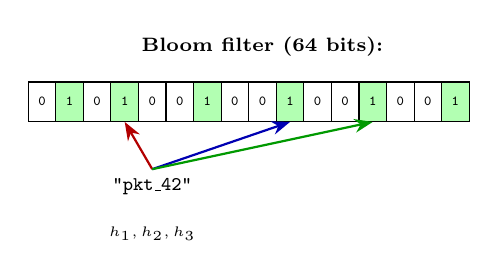
\begin{tikzpicture}[
    >=Stealth,
    bit/.style={draw, minimum width=0.35cm, minimum height=0.5cm,
                font=\tiny\ttfamily}
  ]
  % Bit array
  \node[font=\scriptsize\bfseries] at (2.8, 1.2) {Bloom filter (64 bits):};
  \foreach \x/\v/\c in {
    0/0/white, 1/1/green!30, 2/0/white, 3/1/green!30,
    4/0/white, 5/0/white, 6/1/green!30, 7/0/white,
    8/0/white, 9/1/green!30, 10/0/white, 11/0/white,
    12/1/green!30, 13/0/white, 14/0/white, 15/1/green!30} {
    \node[bit, fill=\c] (b\x) at (\x*0.35, 0.5) {\v};
  }

  % Hash arrows
  \node[font=\scriptsize, below=0.6cm of b4] (key) {\texttt{"pkt\_42"}};
  \draw[->, thick, red!70!black] (key.north) -- (b3.south);
  \draw[->, thick, blue!70!black] (key.north) -- (b9.south);
  \draw[->, thick, green!60!black] (key.north) -- (b12.south);

  \node[font=\tiny, below=0.15cm of key] {$h_1, h_2, h_3$};
\end{tikzpicture}
\end{center}

\vspace{0.5em}
\begin{alertblock}{Memory Efficiency}
A hash table storing 100 packet IDs (4 bytes each) needs $\geq400$ bytes.\\
A Bloom filter with 1\% false positive rate needs only \textbf{120 bytes}
(960 bits, 7 hashes).\\
\textbf{3$\times$ more efficient} --- and no key storage at all.
\end{alertblock}
\end{column}
\end{columns}
\end{frame}

% ===========================================================================
\section{Data Structure}
% ===========================================================================

\begin{frame}[fragile]{The \texttt{tiku\_kits\_ds\_bloom} Structure}
\begin{columns}[T]
\begin{column}{0.48\textwidth}
\begin{lstlisting}[style=cstyle,
  title={ds/bloom/tiku\_kits\_ds\_bloom.h}]
#ifndef TIKU_KITS_DS_BLOOM_MAX_BITS
#define TIKU_KITS_DS_BLOOM_MAX_BITS 256
#endif

#ifndef TIKU_KITS_DS_BLOOM_MAX_HASHES
#define TIKU_KITS_DS_BLOOM_MAX_HASHES 8
#endif

struct tiku_kits_ds_bloom {
    uint8_t bits[
        TIKU_KITS_DS_BLOOM_MAX_BITS / 8];
    uint16_t n_bits;
    uint16_t n_hashes;
    uint16_t count;
};
\end{lstlisting}

\vspace{0.3em}
\textbf{Memory footprint} (default config):\\
$256/8 + 2 + 2 + 2 = 38$ bytes for 256-bit filter.\\
Tracks approximate set membership with zero key storage.
\end{column}

\begin{column}{0.48\textwidth}
\begin{block}{Design Properties}
\begin{itemize}
  \item \textbf{Bit array:} packed into \texttt{uint8\_t} bytes
  \item \textbf{Multiple hashes:} FNV-1a with seed variation
  \item \textbf{Static allocation:} compile-time maximum size
  \item \textbf{No deletions:} set-only semantics (no clear-bit)
  \item \textbf{Count field:} tracks number of insertions
\end{itemize}
\end{block}

\vspace{0.3em}
\begin{alertblock}{Probabilistic Guarantee}
\begin{itemize}
  \item If \texttt{check()} returns 0: element is \textbf{definitely not} in the set
  \item If \texttt{check()} returns 1: element is \textbf{probably} in the set
  \item False positive rate decreases with more bits and more hashes
\end{itemize}
\end{alertblock}
\end{column}
\end{columns}
\end{frame}

% ===========================================================================
\section{Hash Function}
% ===========================================================================

\begin{frame}[fragile]{FNV-1a with Seed Variation}
\begin{columns}[T]
\begin{column}{0.48\textwidth}
\begin{lstlisting}[style=cstyle,
  title={FNV-1a hash --- one function, k seeds}]
static uint32_t fnv1a_hash(
    const uint8_t *data,
    uint16_t len,
    uint32_t seed)
{
    uint32_t hash = 2166136261u ^ seed;
    uint16_t i;

    for (i = 0; i < len; i++) {
        hash ^= (uint32_t)data[i];
        hash *= 16777619u;
    }
    return hash;
}
\end{lstlisting}

\vspace{0.3em}
\begin{block}{Generating $k$ Hashes}
Instead of $k$ different hash functions, use one FNV-1a
with $k$ different seeds: $\text{seed}_i = i$ for
$i \in \{0, \ldots, k{-}1\}$.
\end{block}
\end{column}

\begin{column}{0.48\textwidth}
\textbf{Why FNV-1a?}
\begin{itemize}
  \item Simple: XOR + multiply per byte
  \item No lookup tables (saves FRAM/Flash)
  \item Good avalanche properties
  \item Deterministic --- same input always produces same output
  \item Seed variation produces independent hash values
\end{itemize}

\vspace{0.5em}
\begin{block}{Bit Position Mapping}
\[
  \text{bit} = \texttt{fnv1a(data, len, seed}_i\texttt{)} \bmod n\_bits
\]
\[
  \text{byte} = \text{bit} / 8, \quad \text{pos} = \text{bit} \bmod 8
\]
\end{block}

\vspace{0.3em}
\begin{alertblock}{MCU Friendly}
No division --- modulo on power-of-two sizes compiles to a
bitwise AND. Even non-power-of-two works with the compiler's
built-in modulo on 16-bit MSP430.
\end{alertblock}
\end{column}
\end{columns}
\end{frame}

% ===========================================================================
\section{API Reference}
% ===========================================================================

\begin{frame}[fragile]{Complete API}
\begin{table}
\centering
\small
\begin{tabular}{@{}lp{8cm}@{}}
\toprule
\textbf{Function} & \textbf{Description} \\
\midrule
\texttt{\_bloom\_init(bf, n\_bits, n\_hashes)}
  & Initialize filter with given bit count and hash count; clears all bits \\
\midrule
\texttt{\_bloom\_add(bf, data, len)}
  & Insert element: hash with $k$ seeds, set $k$ bits \\
\texttt{\_bloom\_check(bf, data, len, \&result)}
  & Query membership: result = 1 if all $k$ bits set, 0 otherwise \\
\midrule
\texttt{\_bloom\_clear(bf)}
  & Reset all bits to 0 and count to 0 (epoch reset) \\
\texttt{\_bloom\_count(bf)}
  & Return number of elements added since last clear \\
\bottomrule
\end{tabular}
\end{table}

\vspace{0.3em}
{\scriptsize All functions are prefixed with \texttt{tiku\_kits\_ds}.
Every function validates pointer arguments and returns \texttt{ERR\_NULL} on failure.}

\begin{alertblock}{No Remove Operation}
Bloom filters do not support element removal. Clearing a bit for one
element could invalidate another element that shares that bit position.
Use \texttt{clear()} for a full epoch reset instead.
\end{alertblock}
\end{frame}

% ===========================================================================
\section{Code Examples}
% ===========================================================================

\begin{frame}[fragile]{Example 1: Wireless Packet Deduplication}
\begin{lstlisting}[style=cstyle,
  title={Reject already-seen packets using a Bloom filter}]
#include "tikukits/ds/bloom/tiku_kits_ds_bloom.h"

struct tiku_kits_ds_bloom pkt_filter;
uint8_t seen;

/* 128-bit filter, 3 hashes: ~2% false positive at 10 insertions */
tiku_kits_ds_bloom_init(&pkt_filter, 128, 3);

/* Incoming packet with 4-byte sequence ID */
uint8_t pkt_id[4] = {0xDE, 0xAD, 0xBE, 0xEF};

/* Check if already seen */
tiku_kits_ds_bloom_check(&pkt_filter, pkt_id, 4, &seen);
if (seen) {
    /* Probably a duplicate --- drop the packet */
    return;
}

/* Not seen before --- process and record */
tiku_kits_ds_bloom_add(&pkt_filter, pkt_id, 4);
process_packet(pkt_id);

/* Periodic epoch reset (e.g., every 60 seconds) */
if (epoch_expired()) {
    tiku_kits_ds_bloom_clear(&pkt_filter);
}
\end{lstlisting}
\end{frame}

% ---------------------------------------------------------------------------
\begin{frame}[fragile]{Example 2: Sensor ID Allowlist}
\begin{columns}[T]
\begin{column}{0.52\textwidth}
\begin{lstlisting}[style=cstyle,
  title={Fast membership check for allowed sensors}]
#include "tiku_kits_ds_bloom.h"

struct tiku_kits_ds_bloom allowlist;
uint8_t allowed;

/* 256-bit filter, 5 hashes */
tiku_kits_ds_bloom_init(
    &allowlist, 256, 5);

/* Register known sensor IDs at boot */
uint8_t id1[] = {0x01, 0x3A};
uint8_t id2[] = {0x02, 0x7F};
uint8_t id3[] = {0x03, 0xB1};
tiku_kits_ds_bloom_add(
    &allowlist, id1, 2);
tiku_kits_ds_bloom_add(
    &allowlist, id2, 2);
tiku_kits_ds_bloom_add(
    &allowlist, id3, 2);

/* Check incoming sensor data */
uint8_t incoming[] = {0x04, 0xFF};
tiku_kits_ds_bloom_check(
    &allowlist, incoming, 2, &allowed);
/* allowed == 0: reject unknown sensor */
\end{lstlisting}
\end{column}

\begin{column}{0.44\textwidth}
\begin{center}
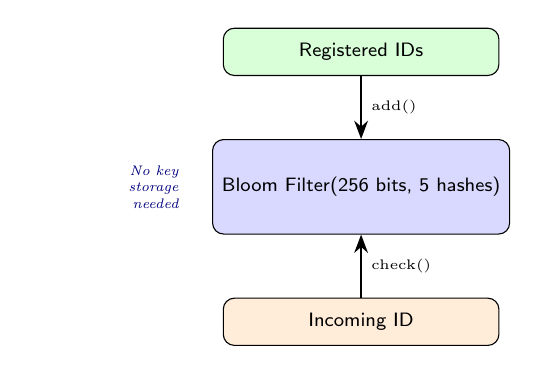
\begin{tikzpicture}[>=Stealth, node distance=0.5cm]
  \node[draw, rounded corners, fill=green!15,
        minimum width=3.5cm, minimum height=0.6cm,
        font=\scriptsize\sffamily] (reg) {Registered IDs};
  \node[draw, rounded corners, fill=blue!15,
        minimum width=3.5cm, minimum height=1.2cm,
        font=\scriptsize\sffamily, below=0.8cm of reg] (bf)
    {Bloom Filter\\(256 bits, 5 hashes)};
  \node[draw, rounded corners, fill=orange!15,
        minimum width=3.5cm, minimum height=0.6cm,
        font=\scriptsize\sffamily, below=0.8cm of bf] (chk)
    {Incoming ID};

  \draw[->, thick] (reg) -- node[right, font=\tiny] {add()} (bf);
  \draw[->, thick] (chk) -- node[right, font=\tiny] {check()} (bf);

  \node[left=0.3cm of bf, font=\tiny\itshape, text=blue!50!black,
        text width=1.8cm, align=right] {No key\\storage\\needed};
\end{tikzpicture}
\end{center}

\vspace{0.5em}
\begin{block}{Allowlist Pattern}
\begin{itemize}
  \item Add known IDs at boot time
  \item Check each incoming ID in $O(k)$
  \item False positive: occasionally accept unknown ID
  \item False negative: \textbf{never} --- known IDs always pass
\end{itemize}
\end{block}

\begin{alertblock}{No Key Storage}
The filter stores only bits --- the actual IDs are not
retained. Memory usage is independent of key size.
\end{alertblock}
\end{column}
\end{columns}
\end{frame}

% ===========================================================================
\section{Embedded Use Case}
% ===========================================================================

\begin{frame}[fragile]{Use Case: Wireless Deduplication with Epoch Reset}
\begin{columns}[T]
\begin{column}{0.52\textwidth}
\begin{lstlisting}[style=cstyle,
  title={Epoch-based dedup for wireless sensor network}]
#include "tiku_kits_ds_bloom.h"

static struct tiku_kits_ds_bloom dedup;
static uint32_t epoch_start;

#define EPOCH_SECONDS  60
#define DEDUP_BITS    256
#define DEDUP_HASHES    4

void dedup_init(void)
{
    tiku_kits_ds_bloom_init(
        &dedup, DEDUP_BITS, DEDUP_HASHES);
    epoch_start = tiku_clock_seconds();
}

void on_packet_rx(uint8_t *id, uint16_t len)
{
    uint8_t seen;
    /* Epoch reset: clear filter periodically */
    if (tiku_clock_seconds() - epoch_start
        >= EPOCH_SECONDS) {
        tiku_kits_ds_bloom_clear(&dedup);
        epoch_start = tiku_clock_seconds();
    }

    tiku_kits_ds_bloom_check(
        &dedup, id, len, &seen);
    if (seen) return;  /* duplicate */

    tiku_kits_ds_bloom_add(
        &dedup, id, len);
    forward_packet(id, len);
}
\end{lstlisting}
\end{column}

\begin{column}{0.44\textwidth}
\begin{center}
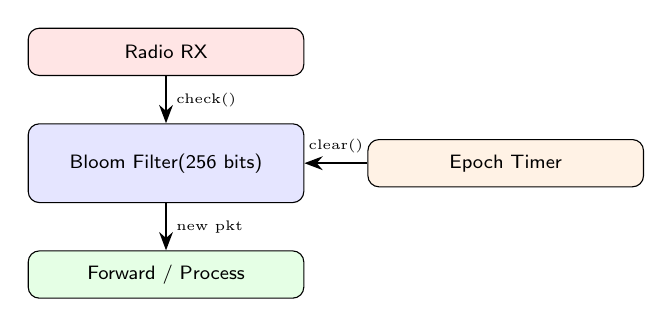
\begin{tikzpicture}[>=Stealth, node distance=0.6cm]
  \node[draw, rounded corners, fill=red!10,
        minimum width=3.5cm, minimum height=0.6cm,
        font=\scriptsize\sffamily] (rx) {Radio RX};
  \node[draw, rounded corners, fill=blue!10,
        minimum width=3.5cm, minimum height=1cm,
        font=\scriptsize\sffamily, below=0.6cm of rx] (bf)
    {Bloom Filter\\(256 bits)};
  \node[draw, rounded corners, fill=green!10,
        minimum width=3.5cm, minimum height=0.6cm,
        font=\scriptsize\sffamily, below=0.6cm of bf] (fwd)
    {Forward / Process};
  \node[draw, rounded corners, fill=orange!10,
        minimum width=3.5cm, minimum height=0.6cm,
        font=\scriptsize\sffamily, right=0.8cm of bf] (clr)
    {Epoch Timer};

  \draw[->, thick] (rx) -- node[right, font=\tiny] {check()} (bf);
  \draw[->, thick] (bf) -- node[right, font=\tiny] {new pkt} (fwd);
  \draw[->, thick] (clr) -- node[above, font=\tiny] {clear()} (bf);
\end{tikzpicture}
\end{center}

\vspace{0.5em}
\begin{block}{Why Epoch Reset?}
\begin{itemize}
  \item Bloom filters fill up over time
  \item False positive rate increases with insertions
  \item Periodic clear bounds the false positive rate
  \item Old packet IDs naturally expire with the epoch
\end{itemize}
\end{block}

\begin{alertblock}{256 bits = 32 bytes}
Entire deduplication state for a 60-second window
fits in 38 bytes total (32 bits array + 6 metadata).
A hash table would need hundreds of bytes.
\end{alertblock}
\end{column}
\end{columns}
\end{frame}

% ===========================================================================
\section{Memory Layout}
% ===========================================================================

\begin{frame}{Memory Layout and False Positive Rate}
\begin{columns}[T]
\begin{column}{0.48\textwidth}
\begin{center}
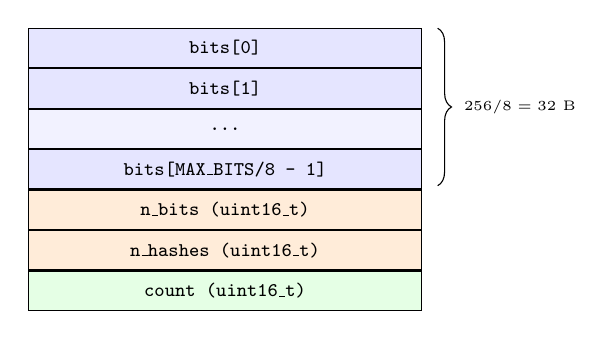
\begin{tikzpicture}[>=Stealth, node distance=0.0cm]
  \node[draw, minimum width=5cm, minimum height=0.5cm,
        fill=blue!10, font=\scriptsize\ttfamily] (b0) {bits[0]};
  \node[draw, minimum width=5cm, minimum height=0.5cm,
        fill=blue!10, font=\scriptsize\ttfamily, below=0cm of b0] (b1) {bits[1]};
  \node[draw, minimum width=5cm, minimum height=0.5cm,
        fill=blue!5, font=\scriptsize\ttfamily, below=0cm of b1] (bd) {...};
  \node[draw, minimum width=5cm, minimum height=0.5cm,
        fill=blue!10, font=\scriptsize\ttfamily, below=0cm of bd] (bn) {bits[MAX\_BITS/8 - 1]};
  \node[draw, minimum width=5cm, minimum height=0.5cm,
        fill=orange!15, font=\scriptsize\ttfamily, below=0cm of bn] (nb) {n\_bits (uint16\_t)};
  \node[draw, minimum width=5cm, minimum height=0.5cm,
        fill=orange!15, font=\scriptsize\ttfamily, below=0cm of nb] (nh) {n\_hashes (uint16\_t)};
  \node[draw, minimum width=5cm, minimum height=0.5cm,
        fill=green!10, font=\scriptsize\ttfamily, below=0cm of nh] (ct) {count (uint16\_t)};

  \draw[decorate, decoration={brace, amplitude=5pt}]
    (2.7, 0.25) -- (2.7, -1.75)
    node[midway, right=6pt, font=\tiny] {$256/8 = 32$ B};
\end{tikzpicture}
\end{center}

\vspace{0.3em}
\begin{block}{Size Formula}
\[
  \text{Total} = \frac{\texttt{MAX\_BITS}}{8} + 6 \text{ bytes}
\]
\end{block}
\end{column}

\begin{column}{0.48\textwidth}
\begin{block}{False Positive Rate}
\[
  p \approx \left(1 - e^{-kn/m}\right)^k
\]
where $m$ = bits, $k$ = hashes, $n$ = insertions.
\end{block}

\begin{table}
\centering
\scriptsize
\begin{tabular}{@{}rrrr@{}}
\toprule
\textbf{Bits ($m$)} & \textbf{Hashes ($k$)} & \textbf{Items ($n$)} & \textbf{FP Rate} \\
\midrule
64   & 3 & 10  & $\sim$4.5\% \\
128  & 3 & 10  & $\sim$0.6\% \\
128  & 5 & 20  & $\sim$2.1\% \\
256  & 4 & 20  & $\sim$0.1\% \\
256  & 5 & 50  & $\sim$2.4\% \\
\bottomrule
\end{tabular}
\end{table}

\vspace{0.3em}
\begin{alertblock}{Optimal Hash Count}
For a given $m/n$ ratio, the optimal number of hashes is:
\[
  k_{\text{opt}} = \frac{m}{n} \cdot \ln 2 \approx 0.693 \cdot \frac{m}{n}
\]
\end{alertblock}
\end{column}
\end{columns}
\end{frame}

% ===========================================================================
\section{Complexity}
% ===========================================================================

\begin{frame}{Time and Space Complexity}
\begin{table}
\centering
\begin{tabular}{@{}lcc@{}}
\toprule
\textbf{Operation} & \textbf{Best Case} & \textbf{Worst Case} \\
\midrule
\texttt{init}   & $O(m/8)$ & $O(m/8)$ \\
\texttt{add}    & $O(k \cdot L)$ & $O(k \cdot L)$ \\
\texttt{check}  & $O(k \cdot L)$ & $O(k \cdot L)$ \\
\texttt{clear}  & $O(m/8)$ & $O(m/8)$ \\
\texttt{count}  & $O(1)$ & $O(1)$ \\
\bottomrule
\end{tabular}
\end{table}

\vspace{0.3em}
{\scriptsize $m$ = number of bits, $k$ = number of hashes, $L$ = length of input data in bytes.}

\vspace{0.5em}
\begin{columns}[T]
\begin{column}{0.48\textwidth}
\begin{block}{Time Analysis}
\begin{itemize}
  \item \texttt{add} and \texttt{check} compute $k$ FNV-1a hashes,
        each iterating over $L$ input bytes
  \item For fixed-size keys (e.g., 4-byte packet IDs), $L$ is constant
  \item \texttt{check} can short-circuit on first unset bit
  \item Total: $O(k)$ for fixed-size keys
\end{itemize}
\end{block}
\end{column}

\begin{column}{0.48\textwidth}
\begin{block}{Space Analysis}
\begin{itemize}
  \item Bit array: $m/8$ bytes
  \item Metadata: 6 bytes (fixed)
  \item Independent of number of elements stored
  \item Independent of key size
  \item 256 bits = 38 bytes total
\end{itemize}
\end{block}
\end{column}
\end{columns}
\end{frame}

% ===========================================================================
\section{Test Suite}
% ===========================================================================

\begin{frame}{Test Cases Overview}
\begin{table}
\centering
\small
\begin{tabular}{@{}clp{7cm}@{}}
\toprule
\textbf{\#} & \textbf{Test Function} & \textbf{What It Verifies} \\
\midrule
1 & \texttt{test\_kits\_ds\_bloom\_init}
  & Initialization, all bits zero, parameter validation \\
2 & \texttt{test\_kits\_ds\_bloom\_add\_check}
  & Add element then check returns 1; unknown returns 0 \\
3 & \texttt{test\_kits\_ds\_bloom\_multiple\_keys}
  & Multiple insertions, all found, non-inserted not found \\
4 & \texttt{test\_kits\_ds\_bloom\_clear}
  & Clear resets all bits, check returns 0, count resets \\
5 & \texttt{test\_kits\_ds\_bloom\_count\_tracking}
  & Count increments on add, resets on clear \\
6 & \texttt{test\_kits\_ds\_bloom\_false\_positive}
  & Validates false positive rate stays below theoretical bound \\
7 & \texttt{test\_kits\_ds\_bloom\_boundary}
  & 8-bit and MAX\_BITS filters, edge-case hash positions \\
8 & \texttt{test\_kits\_ds\_bloom\_null\_inputs}
  & All functions reject NULL with ERR\_NULL \\
\bottomrule
\end{tabular}
\end{table}
\end{frame}

% ===========================================================================
\section{Summary}
% ===========================================================================

\begin{frame}{Summary}
\begin{columns}[T]
\begin{column}{0.48\textwidth}
\begin{block}{What We Built}
\begin{itemize}
  \item Probabilistic set membership filter
  \item Bit array + FNV-1a with seed variation
  \item 5 API functions: init, add, check, clear, count
  \item $O(k)$ add and check for fixed-size keys
  \item 38 bytes total for 256-bit filter
\end{itemize}
\end{block}

\begin{block}{Key Design Choices}
\begin{itemize}
  \item Single hash function with seed variation (no code bloat)
  \item No deletion --- clear for epoch reset
  \item Packed \texttt{uint8\_t} bit array (byte-addressable)
  \item Count field tracks insertion volume
  \item Bounds and NULL checking on all operations
\end{itemize}
\end{block}
\end{column}

\begin{column}{0.48\textwidth}
\begin{block}{Use Cases}
\begin{itemize}
  \item Wireless packet deduplication
  \item Sensor ID allowlist / blocklist
  \item Address filtering in mesh networks
  \item Cache existence pre-check
  \item Resource discovery dedup
\end{itemize}
\end{block}

\begin{block}{Files}
\scriptsize
\begin{tabular}{@{}lp{4.5cm}@{}}
Common: & \texttt{ds/tiku\_kits\_ds.h} \\
Header: & \texttt{ds/bloom/tiku\_kits\_ds\_bloom.h} \\
Source: & \texttt{ds/bloom/tiku\_kits\_ds\_bloom.c} \\
Tests:  & \texttt{tests/ds/test\_kits\_ds\_bloom.c} \\
\end{tabular}
\end{block}
\end{column}
\end{columns}
\end{frame}

% ---------------------------------------------------------------------------
\begin{frame}{Thank You}
\begin{center}
\Large\textbf{TikuKits DS: Bloom Filter}\\[0.5em]
\normalsize Probabilistic Set Membership for Physical AI Endpoints\\[1.5em]

\begin{tabular}{rl}
  Repository: & \url{https://github.com/tikuos/tikuOS} \\
  License:    & Apache 2.0 \\
  Common:     & \texttt{tikukits/ds/tiku\_kits\_ds.h} \\
  Header:     & \texttt{tikukits/ds/bloom/tiku\_kits\_ds\_bloom.h} \\
  Source:     & \texttt{tikukits/ds/bloom/tiku\_kits\_ds\_bloom.c} \\
  Tests:      & \texttt{tikukits/tests/ds/test\_kits\_ds\_bloom.c} \\
\end{tabular}
\end{center}
\end{frame}

\end{document}
